\chapter{heVtAvxBAsagaLu {\rm (fallacies)}}

\section*{virodhABAsagaLalilx eraDu vidha}

\begin{itemize}
\item[{\rm 1)}] {\bf viroVdhoVkitxgaLu} {\rm (Antinomes)}
\item[{\rm 2)}] {\bf heVtAvxBAsagaLu} {\rm (fallacies)}
\end{itemize}

viroVdhoVkitxgaLu eMdareVnu?

tAkiRkavAgi niduRSaTxvAgiruva (Unavilalxda) vAdagaLiMda huTuTxva viroVdhA\-BAsagaLanunx viroVdhoVkitxgaLu eMdu kareyutetxVve.

Iga heVtAvxBAsagaLu eMdareVnu? tiLiyoVNa

takaRbadadhxvAdagaLiMda sAthxpisidaMte meVlf noVTakekx kaMDubaMdarU punaH vimaSiRsidAga vAdadalilx doVSaviruvudanunx nAvu kANabahudu. ivu parasapxra virudadhxvAgiyU, anathaRvAgiyU kANuva sidAdhxMtagaLu.

gaNita shAsatxrXvu karAruvAkAkxda shAsatxrX, AdudariMda I shAsatxrXdalilx baruva sidAdhxMta\-gaLa nirUpaNe niKaravAgiyU, sapxSaTxvAgiyU irabeVkeMdu nAvu niriVkiSxsutetxVve Adare I shAsatxrXdalilxyU viroVdhABAsagaLanunx nAvu noVDabahudu.

biVja gaNitadalilx {\rm 0} yiMda oMdu saMKeyx athavA biVjarAshiyanunx BAgisidAga mAtarx iMtaha heVtAvxBAsagaLanunx nAvu kANabahudu. AdadxriMda {\rm 0} yiMda saMKeyx gaLanunx biVja rAshigaLanUnx BAgisabAradu idara kAraNa tiLiyabeVkAdare BAgAkAra kirxyeya athaRvanunx sariyAgi tiLiyuvudu atAyxvashayxka.

\textbf{udAharaNege:} {\rm 18} nunx {\rm 6} riMda BAgisuvudu eMbudara athaRveVnu? aMdare {\rm 6}~nunx yAva saMKeyxyiMda guNisidAda {\rm 18} kekx samanAguvudoV A saMKeyxyanunx paDeyuvudu. {\rm 18} nunx {\rm 6} riMda BAgisidAga baruva saMKeyxyanunx BAgalabadhx eMdu kareyutetxVve.
\begin{center}
$18\div 6=3$ \quad athavA \quad $\dfrac{18}{6}=3$

$6\times3=18$

sAmAnayxvAgi \quad $b\cdot x=a$ \quad Adare \quad $\dfrac{a}{b}=x$
\end{center}

Iga $\dfrac{18}{0}$ athavA $18\div 0$ eMbudara athaRveVnu? {\rm 0} yanunx yAvudariMda guNisidare {\rm 18} kekx samanAguvudoV A saMKeyxyanunx paDeyuvudu.

 $a$ eMbudu yAva vAsatxva saMKeyxyeV Agirali
\begin{center}
$0\times a=0$
\end{center}
AdudariMda {\rm 0} nunx yAva saMKeyxyiMda guNisidarU guNalabadxvu {\rm 0} yeV Aguvudu. {\rm 18} Aguvududilalx AdudariMda {\rm 18} nunx {\rm 0} yiMda BAgisidAga BAgalabadhxvilalx eMdare $\dfrac{18}{0}$ eMbudakekx athaRvilalx. sAmAnayxvAgi $a$ eMbudu shUnayxkikxMta BinanxvAda yAva saMKeyxyeV Agirali $\dfrac{a}{0}$ eMbudakekx athaRvilalx AdudariMda {\rm 0} yiMda  saMKeyxgaLanunx athavA biVjarAshiyanunx BAgisabAradu.
\begin{gather*}
0\times 4=0; \quad 0\times 6=0\tag{\rm 1}\\
\therefore \quad 0\times 4=0\times 6 \quad \tag{\rm 2}\\
\therefore \quad 4=6 \quad \tag{\rm 3}  
\end{gather*}
idu oMdu viroVdhABAsa {\rm 4} eMbudu {\rm 6} kekx samanAgalu sAdhayxvilalx\break 
I viroVdhABAsavu baralu kAraNaveVnu? eraDaneya {\rm (2)} samiVkaraNada eraDu kaDeyanUnx {\rm 0} yiMda BAgisidedxVve. idu sariyalalx aMdare ililx nAvu {\rm 0} yiMda eraDu kaDeyanUnx BAgisidedxVve. idariMda viroVdhABAsagaLu uMTAyitu matotxMdu udAharaNe noVDoVNa.
\begin{center}
$a=3 ; b=2$ \quad matutx \quad $c=5$ \quad AdAga

$3+2=5$

aMdare \quad $a+b=c$

$(a+b)(a+b)=(a+b)c$
\end{center}
(samiVkaraNada eraDu kaDegaLanUnx $(a+b)$ yiMda guNiside)
\begin{align*}
\therefore \quad a^2+2ab&+b^2=ac+bc\\
a^2+ab-ac&=-ab-b^2+bc\\
a(a+b-c)&=-b(a+b-c)
\end{align*}
Iga samiVkaraNada eraDu kaDeyanUnx $(a+b-c)$ yiMda BAgisidare
\begin{align*}
a&=-b\\
\therefore \quad 3&=-2
\end{align*}
idu oMdu viroVdhABAsa

$(a+b-c)=0$ \quad EkeMdare \quad $a+b=-c$

$(a+b-c)$ iMda samiVkaraNada eraDu kaDeyanUnx BAgisidAga nAvu {\rm 0} yiMda BAgisidaMtAyitu.

{\bf I udAharaNe noVDi}

obabxnige aidaneya huTiTxda hababxda dina ipapxtutx vaSaR vayasusx tuMbitaMte idu meVlf noVTakekx viroVdhABAsavAgi kaMDubaMdarU, I heVLikeyalilx yAva\break viroVdhavU ilalx. EkeMdare avanu Pebarxvari ipapxtotxMbatatxneya tAriVKina dina\break huTiTxdudx. huTiTxda hababxgaLanunx vaSaRdalilx AyAtiMgaLa, AyA tAriVKige anuguNa\-vAgi oMdu deVshadalilx AcarisutAtxre (yUroVpf) parxti vaSaRvU Pebarxvariyalilx {\rm 29} dinagaLu iruvudilalx. sAmAnayxvAgi parxtivaSaRvU Pebarxvari tiMgaLinalilx {\rm 28} neV tAriVKu koneyadu. muMdina dinaveV mAciR oMdaneV tAriVKu nAlukx vaSaRgaLigomemx mAtarx Pebarxvari {\rm 29} dinagaLu barutatxde. huTiTxda hababx Acarisi koMDavana eraDaneya huTiTxda hababx baruvudeV avanu huTiTxda nAlukxvaSaRgaLige. parxtinAlukx vaSaRgaLigomemx huTiTxda hababxvanunx avanu AcarisabeVkAgiruvudariMda aidaneya huTiTxda hababxda dina ipapxtutx vaSaRvayasusx Agiruvudaralilx AshacxyaRveVnU kaMDubaruvudilalx. matotxMdu udAharaNeyanunx noVDoVNa.

citarxvanunx sariyAgi gamanisi.
\begin{figure}[H]
\centering
\includegraphics{src/figures/083.eps}
\end{figure}

meVlina citarxdalilx cakarxvu $A$ yiMda $B$ ge uruLuvAga (calisuvAga) adu saMpUNaRvAgi oMdu sututx sutitxde. AdudariMda $AB$ ya udadx cakarxda paridhige sama cakarxda oLa meVlemxYya meVliruva $C$ biMduvu oMdu saNaNxvaqtatxda paridhiya meVlide cakarxvu oMdu sututx sututxva kAladalilxyeV $C$ biMdu iruva vaqtatxvU oMdu sututx sutitx, A biMdu $D$ eMba sAthxnakekx baMdide AdudariMda $CD$ ya udadx saNaNx vaqtatxda paridhige samanAgirabeVku. Adare citarxvanunx gamanaviTuTx noVDidAga $CD=AB$. AdudariMda $C$ biMduvu iruva saNaNx vaqtatxda paridhiyu $A$ biMduviruva doDaDx vaqtatxda paridhige sama eMba viroVdhABAsavanunx opapxbeVkAgutatxde.

savxlapx vimasheR mADi noVDidAga I viroVdha bagehariyutatxde.

cakarxvu $A$ yiMda $B$ ge uruLuvAga, adara oLameVlemxYya meVle iruva $C$ biMduvu keVMdarxda sutatxlU tirugutAtx saNaNx vaqtatxda paridhiya meVle saMcarisuvudu nija. jotege $C$ biMduvanunx cakarxvu $A$ yiMda $B$ ya kaDege eLeyutatxlU ide. cakarxda keVMdarx $P$ yiMda $Q$ biMduvige baMdiruva karxmavanunx noVDidare I viSaya namage inUnx sapxSaTxvAgutatxde. cakarxvu uruLutAtx $A$ yiMda $B$ ge hoVguvAga $P$ biMduvanunx $Q$ biMduvige eLedukoMDu hoVgide. idariMda noVTakekx $AB$ ya dUra $CD$ dUrakekx samaveMdu kANisutatxde. 

jiZno {\rm (Zeno)} eMba hesarAMta vayxkitx parxtipAdisida matotxMdu viroVdhABAsaveMdare akilisf matutx Amege saMbaMdhisidudx.

akilisfgU, oMdu AmegU oMdu oMdu bAri OTada sapxdheR naDeyitu enonxVNa. Ameya hatatxraSuTx veVga akilisanigide eMdu BAvisoVNa Ameyu ODuva veVga kaDimeyAdadxriMda sapxdheRya AraMBadalilx Ameyanunx nUrugaja muMde iDuvaMte (hiMde idadx birxTiSf padadhxti) tiLisidanaMte. sapxdheRyu AraMBavAdAga citarxdalilx tiLisiruvaMte Ameyu $T$ eMba jAgadalilxyU (sathxLa) akilisanu $A$ eMba sathxLadalUlx idadxru. 
\begin{figure}[H]
\centering
\includegraphics[scale=.8]{src/figures/m_085.eps}
\end{figure}


sapxdheRyu AraMBavAyitu. akilisanu AmeyiMda nUrugaja hiMde iruvudariMda I nUrugajada dUrada mUlaka akilisanu muMce ODaleVbeVku. akilisana veVga Ameya veVgada hatatxraSuTx athavA Ameya veVga akilisana veVgada hatatxneya oMdu BAgakekx sama eMdare oMdu gotAtxda kAlada avadhiyalilx akilisanu eSuTx dUra hoVgirutAtxnoV adara hatatxneya oMdu BAgadaSuTx dUra muMdakekx Ameyu hoVgirutatxde. akilisanu nUru gaja ODuva kAladalilx Ameyu hatutx gaja muMdirutatxde. aMkilisanu I hatutxgaja hoVguvudaroLage Ameyu oMdu gaja ({\rm 1} gaja) muMdiruvudu akilisanu I oMdu gaja ({\rm 1} gaja) ODuvudaroLage Ameyu $\dfrac{1}{10}$ gaja muMdirutatxde. akilisanu I $\dfrac{1}{10}$ gaja ODuvudaroLage Ameyu akilisanigiMta $\frac{1}{100}$ gaja muMdirutatxde. hiVge anaMtara yAva kAladalelxV Agali Ameyu akilisanigiMta savxlapxvAdarU muMdeyeV irutatxde. AdudariMda Ameyanunx soVlisalu akilisanige sAdhayxvAguvudilalx. sapxdheRyalilx AmeyeV gelulxvudu KaMDita.

idu eMtaha viroVdhABAsa (heVtAvxBAsa) nijavAgiyU iMtaha oMdu OTada sapxdheR naDedidedxV Adare akilisaneV gelulxvudu savxtasidadhx. Adare jiZnoVparxtipAdisiruva vAdadalilx yAva doVSavU kANuvudilalx. I viroVdhABAsavu  jiZnoVvina kAlakekx sari eMdu kaMDididxrabahudu.

Adare gaNita shAsatxrXdalilx ililxya tanaka Agiruva AviSAkxragaLu I viroVdhABAsavanunx (heVtAvxBAsa) pariharisuvaSuTx sAmathayxRvanunx paDedive.

akilisf athavA Ameyu ODuva dUragaLanunx sUcisuva saMKeyxgaLu anaMta padagaLiruva oMdu sherxVNi $100+10+1+\dfrac{1}{10}+\dfrac{1}{100}+\dfrac{1}{1000}\ldots\ldots$anaMta padagaLavarege idu oMdu guNoVtatxra sherxVNi. idara modalaneya pada $a=100$ I sherxVNiya parxtiyoMdu saMKeyxyanUnx $\dfrac{1}{10}$ riMda guNisidAga muMdina saMKeyx barutatxde.

$\therefore$ sherxVNiya sAmAnayx parxmANa $r=\dfrac{1}{10}$ iMtaha sherxVNiya sAmAnayx parxmANa {\rm 1} kikxMta kaDimeyAdAga anaMta padagaLa motatx $=\dfrac{a}{1-r}$
$$
\frac{100}{1-\frac{1}{10}}=\frac{100}{\frac{9}{10}}=100\times \frac{10}{9}=\frac{1000}{9}=111\frac{1}{9}
$$
aMdare akilisf athavA Ame ivu ODuva dUragaLelalxvanUnx kUDisidAga $111\dfrac{1}{9}$ gajakekx samanAguvudu.

akilisf matutx Ame ivarugaLa OTada sapxdheR anaMtavAda haMtagaLalilx naDeyalilalx modalu $100$ gaja ODi anaMtara $10$ gaja, anaMtara $1$, anaMtara $\dfrac{1}{10}$ anaMtara $\dfrac{1}{100}$ itAyxdi - I riVti haMta haMtagaLalilx ODabeVkeMdu avarige tiLisiralilalx ODuva sapxdheR aviciCxnanxvAgi naDeyitu.

$111\dfrac{1}{9}$ gajada dUravanunx anaMta BAgagaLAgi viBajisi haMta haMtagaLalilx OTada sapxdheRyu naDedaMte BAvisi vAda mADidadxriMda viroVdhavidadxMte kaMDitu. 

akilisf matutx Ame - ivara OTada sapxdheR oMdu niyatavAda kAlada avadhiyalilx mugidirutatxde. sapxdheRya avadhiyalilx akilisanu ODuva dUra Ameyu hoVguva dUrakikxMta hecAcxdudariMda akilisanu gelalxlu aDiDx EnU ilalx.

\hfill{-AdhAra}
